\section{Additional results}\label{app:extra}

Table~\ref{tab:tuned} repeats Table~\ref{tab:main} with Optuna-tuned hyper-parameters. Tuning improved the
deployed alarms of the GRU and the Transformer--LSTM and reduced those of the LSTM, CNN-LSTM, TCN and
PatchTST; tuning on a single small calibration well mainly adds variance. Table~\ref{tab:faclass} lists false
alarms per confounder class, Table~\ref{tab:robust} the robustness tests and Table~\ref{tab:v1v2} the
generalisation from 3W version 1.1.1 to version 2.0.0. Figures~\ref{fig:reliab} and~\ref{fig:lead} show the
calibration of the forecasts and the lead times of caught events.

\begin{table*}[t]
\caption{As Table~\ref{tab:main}, with Optuna-tuned hyper-parameters (equal budget, tuned on calibration wells).}\label{tab:tuned}
\scriptsize\setlength{\tabcolsep}{3pt}
\resizebox{\textwidth}{!}{\begin{tabular}{lcccccccccc}
\toprule
Model & Seeds & AUPRC@24h & AUROC@24h & C-index & IBS & ECE & BSS & Rec.@1/mo & Hits/24 & PICP \\
\midrule
{B1 Logistic regression} & 1 & 0.281 & 0.406 & 0.434 & 0.366 & 0.529 & 0.26 & 0.04 & 0 & 0.94 \\
{B2 GBDT} & 1 & 0.662 & 0.893 & 0.786 & 0.081 & 0.217 & 0.68 & 0.71 & 6 & 0.72 \\
{B3 LSTM} & 1 & 0.776 & 0.917 & 0.855 & 0.103 & 0.197 & 0.72 & 0.12 & 2 & 0.45 \\
{B4 GRU} & 1 & 0.668 & 0.902 & 0.890 & 0.100 & 0.204 & 0.76 & 0.71 & 17 & 0.41 \\
{B5 CNN-LSTM} & 1 & 0.689 & 0.897 & 0.818 & 0.125 & 0.215 & 0.70 & 0.08 & 5 & 0.53 \\
{B6 TCN} & 1 & 0.762 & 0.940 & 0.879 & 0.116 & 0.190 & 0.77 & 0.12 & 7 & 0.46 \\
{B7 Transformer-LSTM$^\dagger$} & 1 & 0.752 & 0.930 & 0.869 & 0.067 & 0.126 & 0.85 & 0.79 & 16 & 0.70 \\
{B8 PatchTST$^\dagger$} & 1 & 0.616 & 0.827 & 0.849 & 0.149 & 0.198 & 0.75 & 0.67 & 11 & 0.53 \\
{B8i iTransformer} & 1 & 0.700 & 0.935 & 0.820 & 0.091 & 0.157 & 0.78 & 0.46 & 14 & 0.60 \\
{B9 LSTM-AE detector$^\dagger$} & 1 & 0.211 & 0.312 & 0.431 & 0.765 & 0.848 & -0.93 & 0.00 & 0 & 0.85 \\
{PI-PatchSurv (ours)} & 5 & 0.596$\pm$0.093 & 0.746$\pm$0.076 & 0.765 & 0.105 & 0.285 & 0.64 & 0.25 & 5.6$\pm$2.9 & 0.86 \\
\bottomrule
\end{tabular}}
\footnotetext{AUPRC/AUROC and hits: mean$\pm$SD over single-seed runs where several seeds exist; other columns: ensemble of the available seeds. BSS: Brier skill score at 24~h relative to B0. Rec.@1/mo: threshold-free recall at one false alarm per well-month. Hits: events caught out of 24 with the deployed calib-self threshold. PICP: coverage of the 90\,\% conformal interval. $^\dagger$Re-implementation of a base-paper architecture.}
\end{table*}

\begin{table}[t]
\caption{False-alarm episodes per confounder class (calib-self; all real non-scaling instances tested once); $^\ddagger$tuned}\label{tab:faclass}
\scriptsize
\begin{tabular*}{\columnwidth}{@{\extracolsep\fill}lccccc}
\toprule
Class & Inst. & B2 & B4$^\ddagger$ & B7$^\ddagger$ & Ours \\
\midrule
0 normal & 594 & 50 & 0 & 3 & 3 \\
6 quick restr. & 6 & 0 & 0 & 0 & 0 \\
8 hydrate (prod.) & 14 & 3 & 2 & 1 & 21 \\
9 hydrate (serv.) & 57 & 8 & 6 & 3 & 12 \\
3 slugging & 32 & 0 & 0 & 0 & 9 \\
1, 2, 4, 5 & 380 & 4 & 5 & 4 & 2 \\
\bottomrule
\end{tabular*}
\end{table}

\begin{table}[t]
\caption{Robustness (E3): AUPRC@24h under corruptions of the test inputs.}\label{tab:robust}
\scriptsize
\begin{tabular*}{\columnwidth}{@{\extracolsep\fill}lcc}
\toprule
Condition & PI-PatchSurv & B3 LSTM \\
\midrule
clean & 0.697 & 0.811 \\
Gaussian noise 1\,\% & 0.696 & 0.808 \\
Gaussian noise 3\,\% & 0.683 & 0.793 \\
Gaussian noise 5\,\% & 0.674 & 0.773 \\
1 sensor dropped & 0.714 & 0.682 \\
2 sensors dropped & 0.725 & 0.613 \\
3 sensors dropped & 0.700 & 0.564 \\
1 sensor frozen 60 min & 0.699 & 0.796 \\
resampled to 30 s & 0.653 & 0.824 \\
resampled to 60 s & 0.635 & 0.814 \\
resampled to 120 s & 0.611 & 0.787 \\
resampled to 300 s & 0.581 & 0.765 \\
\bottomrule
\end{tabular*}
\end{table}

\begin{table}[t]
\caption{Generalisation: trained on wells of 3W v1.1.1, tested on wells added in v2.0.0 (20 events)}\label{tab:v1v2}
\scriptsize
\begin{tabular}{lccc}
\toprule
Model & AUPRC@24h & AUROC@24h & Hits/20 / FA \\
\midrule
B0 & 0.194 & 0.704 & 0 / 0.261 \\
B2 & 0.227 & 0.693 & 2 / 0.174 \\
B3 & 0.475 & 0.834 & 3 / 0.112 \\
B4 & 0.358 & 0.690 & 9 / 0.050 \\
B5 & 0.339 & 0.776 & 0 / 0.062 \\
B6 & 0.185 & 0.702 & 0 / 0.075 \\
B7 & 0.166 & 0.683 & 0 / 0.000 \\
B8 & 0.605 & 0.922 & 1 / 0.485 \\
B8i & 0.264 & 0.822 & 0 / 0.137 \\
B9 & 0.097 & 0.447 & 0 / 0.050 \\
PI-PatchSurv & 0.278 & 0.841 & 4 / 0.373 \\
\bottomrule
\end{tabular}
\end{table}


\begin{figure}[t]
\centering
\begin{minipage}{0.46\textwidth}
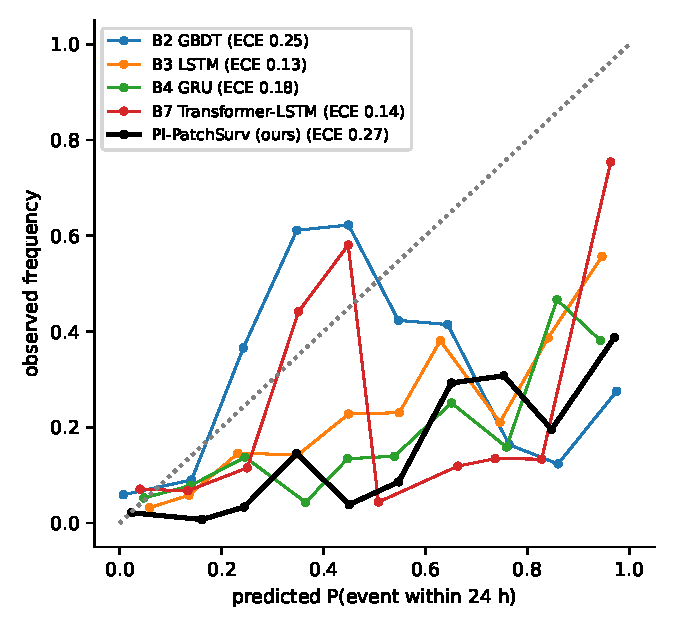
\includegraphics[width=\linewidth]{figures/reliability_24h.pdf}
\caption{Reliability diagram for an event within 24~h (pooled test wells) with the expected calibration error}
\label{fig:reliab}
\end{minipage}\hfill
\begin{minipage}{0.52\textwidth}
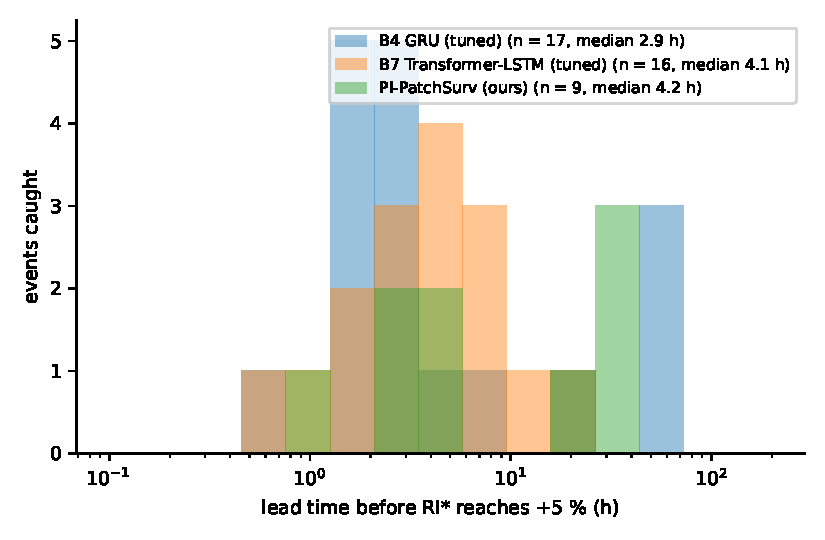
\includegraphics[width=\linewidth]{figures/lead_time_hist.pdf}
\caption{Lead time of caught events under the deployed self-referenced threshold}
\label{fig:lead}
\end{minipage}
\end{figure}

\section{Reproducibility details}\label{app:repro}

Table~\ref{tab:repro} lists the settings needed to reproduce the experiments.

\begin{table}[h]
\caption{Settings used in all experiments}
\label{tab:repro}
\footnotesize
\begin{tabular*}{\textwidth}{@{\extracolsep\fill}p{2.2cm}p{9.8cm}}
\toprule
Item & Setting \\
\midrule
Data & 3W v2.0.0, commit \texttt{826fec4}; onset = first label 107 or 7; event when the 60-min rolling median of $\RI$ reaches 1.05; windows of 360~min every 10~min; horizons 1, 3, 6, 12, 24 and 72~h \\
Splits & Six leave-one-well-out folds (test wells 1, 6, 21, 22, 23, 24); calibration well = next scaling well with an event, never well 24; non-scaling wells rotate into test and calibration groups; v1$\to$v2: train on wells 1, 6 and 21, test on 22--24, calibrate on 6 \\
Hyper-parameters & $d=64$; AdamW, learning rate $10^{-3}$, weight decay $10^{-4}$; batch 256; 12 epochs of 150 steps; dropout 0.1; Transformer with 2 layers, 4 heads, feed-forward width 128; patch 16, stride 8; $\lambda=0.1$; recurrent baselines with 2 layers \\
Tuning & Optuna 5.0, TPE sampler (seed 0), median pruner, 20 trials per fold, 4 epochs per trial; learning rate $[10^{-4},3\cdot10^{-3}]$ (log), weight decay $[10^{-6},10^{-2}]$ (log), batch $\{128,256,512\}$, $\lambda\in[0,0.5]$ (PI-PatchSurv) \\
Seeds & 0--4 for PI-PatchSurv, its \emph{-SI} and tuned variants; 0--2 for deep baselines and the physics, survival-head and synthetic-data ablations; 0 for other variants \\
Environment & Python 3.14.7, PyTorch 2.15.0, NumPy 2.5, pandas 3.1, scikit-learn 1.9.1, SciPy 1.18, Optuna 5.0; Apple M4 (MPS, float32) and Kaggle with two NVIDIA T4 GPUs (CUDA) \\
Commands & \texttt{python experiments/analyze.py}, \texttt{python experiments/analyze.py --split v1v2} and \texttt{python scripts/paper\_tables.py} regenerate all tables and figures; \texttt{scripts/phase2\_queue.sh} runs the full training pipeline \\
\botrule
\end{tabular*}
\end{table}
